\begin{frame}[fragile]{OJ 216 -- Getting in Line}

{\it Computer networking requires that the computers in the network be linked.

This problem considers a ``linear'' network in which the computers are chained together so that each
is connected to exactly two others except for the two computers on the ends of the chain which are
connected to only one other computer. A picture is shown below. Here the computers are the black
dots and their locations in the network are identified by planar coordinates (relative to a coordinate
system not shown in the picture).

Distances between linked computers in the network are shown in feet.}
\end{frame}


\begin{frame}[fragile]{OJ 216 -- Getting in Line}
\begin{figure}[h]
    \centering

    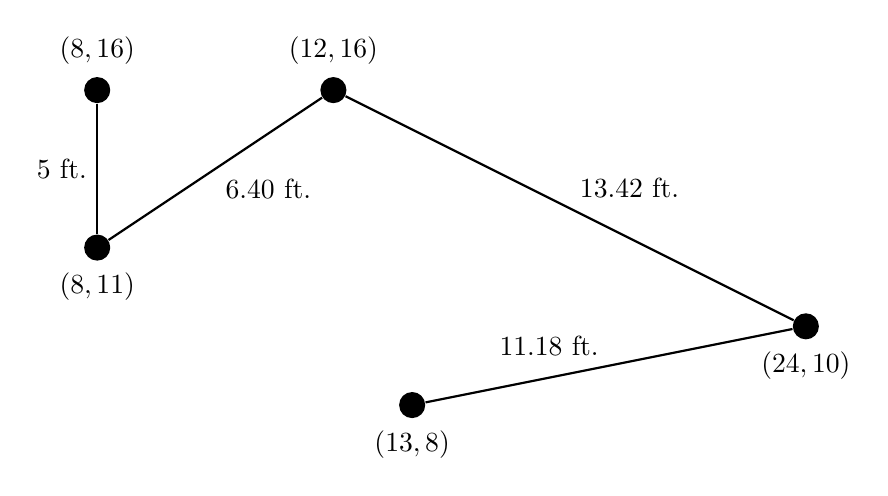
\begin{tikzpicture}
        \node[circle,fill] (A) at (0, 4) { };
        \node[circle,fill] (B) at (0, 2) { };
        \node[circle,fill] (C) at (3, 4) { };
        \node[circle,fill] (D) at (9, 1) { };
        \node[circle,fill] (E) at (4, 0) { };

        \node at (0, 4.5) { $(8, 16)$ };
        \node at (0, 1.5) { $(8, 11)$ };
        \node at (3, 4.5) { $(12, 16)$ };
        \node at (9, 0.5) { $(24, 10)$ };
        \node at (4, -0.5) { $(13, 8)$ };

        \draw[thick] (A) to node[left] { 5 ft. } (B);
        \draw[thick] (B) to node[below right] { 6.40 ft. } (C);
        \draw[thick] (C) to node[above right] { 13.42 ft. } (D);
        \draw[thick] (D) to node[above left] { 11.18 ft. } (E);
    \end{tikzpicture}
\end{figure}

\end{frame}

\begin{frame}[fragile]{OJ 216 -- Getting in Line}

{\it For various reasons it is desirable to minimize the length of cable used.

Your problem is to determine how the computers should be connected into such a chain to minimize
the total amount of cable needed. In the installation being constructed, the cabling will run beneath
the floor, so the amount of cable used to join $2$ adjacent computers on the network will be equal to
the distance between the computers plus $16$ additional feet of cable to connect from the floor to the
computers and provide some slack for ease of installation.

The picture below shows the optimal way of connecting the computers shown above, and the total
length of cable required for this configuration is $(4+16)+ (5+16) + (5.83+16) + (11.18+16) = 90.01$
feet.}

\end{frame}

\begin{frame}[fragile]{OJ 216 -- Getting in Line}
\begin{figure}[h]
    \centering

    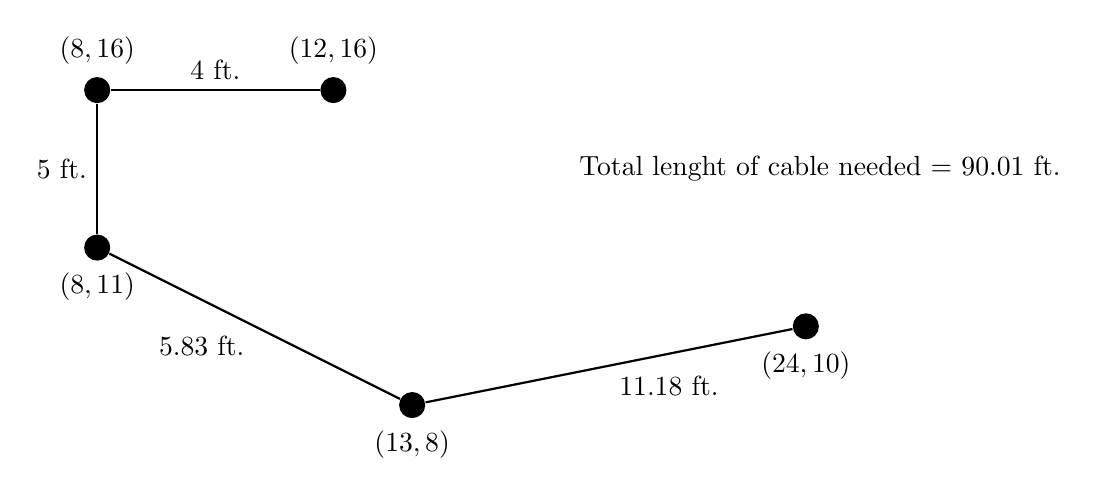
\begin{tikzpicture}
        \node[circle,fill] (A) at (0, 4) { };
        \node[circle,fill] (B) at (0, 2) { };
        \node[circle,fill] (C) at (3, 4) { };
        \node[circle,fill] (D) at (9, 1) { };
        \node[circle,fill] (E) at (4, 0) { };

        \node at (0, 4.5) { $(8, 16)$ };
        \node at (0, 1.5) { $(8, 11)$ };
        \node at (3, 4.5) { $(12, 16)$ };
        \node at (9, 0.5) { $(24, 10)$ };
        \node at (4, -0.5) { $(13, 8)$ };
        \node[anchor=west] at (6, 3) { Total lenght of cable needed = $90.01$ ft.};

        \draw[thick] (A) to node[left] { 5 ft. } (B);
        \draw[thick] (A) to node[above] { 4 ft. } (C);
        \draw[thick] (B) to node[below left] { 5.83 ft. } (E);
        \draw[thick] (D) to node[below right] { 11.18 ft. } (E);
    \end{tikzpicture}
\end{figure}

\end{frame}

\begin{frame}[fragile]{Entrada e saída}

\textbf{Input}

{\it The input file will consist of a series of data sets. Each data set will begin with a line consisting of a
single number indicating the number of computers in a network. Each network has at least $2$ and at
most $8$ computers. A value of 0 for the number of computers indicates the end of input.

After the initial line in a data set specifying the number of computers in a network, each additional
line in the data set will give the coordinates of a computer in the network. These coordinates will be
integers in the range $0$ to $150$. No two computers are at identical locations and each computer will be
listed once.}

\end{frame}

\begin{frame}[fragile]{Entrada e saída}

\textbf{Output}

{\it The output for each network should include a line which tells the number of the network (as determined
by its position in the input data), and one line for each length of cable to be cut to connect each adjacent
pair of computers in the network. The final line should be a sentence indicating the total amount of
cable used.

\textbf{In listing the lengths of cable to be cut, traverse the network from one end to the
other}. (It makes no difference at which end you start.) Use a format similar to the one shown in the
sample output, with a line of asterisks separating output for different networks and with distances in
feet printed to $2$ decimal places.}

\end{frame}

\begin{frame}[fragile]{Exemplo de entrada e saída}

\begin{scriptsize}
\begin{minipage}[t]{0.35\textwidth}
\textbf{Entrada}
\begin{verbatim}
6
5 19
55 28
38 101
28 62
111 84
43 116
5
11 27
84 99
142 81
88 30
95 38
3
132 73
49 86
72 111
0
\end{verbatim}
\end{minipage}
\begin{minipage}[t]{0.6\textwidth}
\textbf{Saída}
\begin{verbatim}
**********************************************************
Network #1
Cable requirement to connect (5,19) to (55,28) is 66.80 feet.
Cable requirement to connect (55,28) to (28,62) is 59.42 feet.
Cable requirement to connect (28,62) to (38,101) is 56.26 feet.
Cable requirement to connect (38,101) to (43,116) is 31.81 feet.
Cable requirement to connect (43,116) to (111,84) is 91.15 feet.
Number of feet of cable required is 305.45.
**********************************************************
Network #2
Cable requirement to connect (11,27) to (88,30) is 93.06 feet.
Cable requirement to connect (88,30) to (95,38) is 26.63 feet.
Cable requirement to connect (95,38) to (84,99) is 77.98 feet.
Cable requirement to connect (84,99) to (142,81) is 76.73 feet.
Number of feet of cable required is 274.40.
**********************************************************
Network #3
Cable requirement to connect (132,73) to (72,111) is 87.02 feet.
Cable requirement to connect (72,111) to (49,86) is 49.97 feet.
Number of feet of cable required is 136.99.
\end{verbatim}
\end{minipage}
\end{scriptsize}

\end{frame}


\begin{frame}[fragile]{Solução em $O(N\times N!)$ }

    \begin{itemize}
        \item Como o número total de computadores é relativamente pequeno, é possível
            resolver este problemas por meio da enumeração e avaliação de todas as $N!$
            permutações distintas

        \item Cada permutação pode ser avaliada em $O(N)$, de modo que esta solução terá 
            complexidade $O(N\times N!)$

        \item A distância euclidiana entre os pontos $P = (x_P, y_P)$ e $Q = (x_Q, y_Q)$ é dada
            por
        $$
            d(P, Q) = \sqrt{(x_P - x_Q)^2 + (y_P - y_Q)^2}
        $$

        \item É preciso acrescentar, a cada distância entre pares de computadores, 16 metros,
            conforme instrui o texto do problema
    \end{itemize}

\end{frame}

\begin{frame}[fragile]{Solução}
    \inputsnippet{cpp}{5}{22}{codes/216.cpp}
\end{frame}

\begin{frame}[fragile]{Solução}
    \inputsnippet{cpp}{24}{40}{codes/216.cpp}
\end{frame}
